\documentclass[a4paper, 14pt]{extarticle}



\usepackage[main=russian,english]{babel}   %% загружает пакет многоязыковой вёрстки
\usepackage{fontspec}      %% подготавливает загрузку шрифтов Open Type, True Type и др.

\setmainfont{Times New Roman}
\setsansfont{Times New Roman}

\usepackage{icomma}
\usepackage{siunitx}
\usepackage[a4paper,top=1cm,bottom=2cm,left=3cm,right=1.5cm, marginparwidth=2cm]{geometry}

\usepackage{graphicx}
\usepackage{amsmath, amsfonts}
\usepackage{longtable}
\usepackage{icomma}
\usepackage{indentfirst}


\usepackage{mathrsfs}
\usepackage{xcolor}
\usepackage{hyperref}
\usepackage{enumitem}
\usepackage[export]{adjustbox}

\input{../include/definitions.inc}

\begin{document}
	
	
\section{Плоские потенциальные течения идеальной жидкости и комплексные потенциалы}



\subsection{Построение комплексного потенциала плоского потенциального течения идеальной жидкости }

Если возможно ввести систему координат так, что течение идеальной жидкости ($\rho=const$) будет описываться уравнениями:	
\begin{equation}
	\label{eq:ideal_liquid_planar_mass}
	\pd{v_x}{x}+\pd{v_y}{y} = 0,
\end{equation}
\begin{equation}
	\label{eq:ideal_liquid_planar_momentum_x}
	\pd{v_x}{t}+v_x \pd{v_x}{x} + v_y \pd{v_x}{y} = -\frac{1}{\rho} \pd{p}{x},
\end{equation}	
\begin{equation}
	\label{eq:ideal_liquid_planar_momentum_y}
	\pd{v_y}{t}+v_x \pd{v_y}{x} + v_y \pd{v_y}{y} = -\frac{1}{\rho} \pd{p}{y},	
\end{equation}
где $v_x = v_x(t,x,y)$, $v_y = v_y(t,x,y)$, $p=p(t,x,y)$ -- функции, заданные в некоторой исследуемой области, то говорят, что движение идеальной жидкости \textit{плоскопараллельное}.

\begin{dfn}
	Функция $\psi=\psi(x,y)$ такая, что 
	\[
	v_x = \pd{\psi}{y},\quad
	-v_y = \pd{\psi}{x},
	\]
	называется функцией тока. Если течение нестационарное, то $t$ -- дополнительный параметр.
\end{dfn}

Для функции $\psi = \psi(x,y)$ уравнение неразрывности (\ref{eq:ideal_liquid_planar_mass})
\[
	\pd{v_x}{x} + \pd{v_y}{y} = 
	\pd{}{x} \left( \pd{\psi}{y} \right) + \pd{}{y} \left( -\pd{\psi}{x} \right) = 0
\]
выполняется тождественно.


Рассмотрим уравнения \textit{линий тока}:
\[
	\frac{dx}{v_x(x,y)} = \frac{dy}{v_y(x,y)},
\]
тогда
\[
0 = -v_y dx + v_x dy = \pd{\psi}{x} dx + \pd{\psi}{y} dy =  d\psi.
\]
Таким образом, $\psi=\psi(x,y)$ \textit{сохраняет} одно и то же значение \textit{на линиях тока}.
		
Вектор вихря $\vec{\Omega}= \rot \vec{v}$ задается формулами:
\[
	\Omega_x = \pd{v_z}{y}-\pd{v_y}{z} = 0,\quad
	\Omega_y = \pd{v_x}{z}-\pd{v_z}{x} = 0,
\]
\[
	\Omega_z = \pd{v_y}{x}-\pd{v_x}{y} = -\pdk{\psi}{x} - \pdk{\psi}{y}.
\]
		
В случае безвихревого течения ($\vec{\Omega} = 0$):
\[
	\Delta \psi = \pdk{\psi}{x} + \pdk{\psi}{y} = 0.
\]


Если плоское течение идеальной жидкости \textit{потенциально}, тогда существует функция $\varphi(x,y)$ такая, что
\[
	v_x = \pd{\varphi}{x},\quad
	v_y = \pd{\varphi}{y}, 
\]
при этом
\begin{equation}
	\label{eq:Cauchi_Riman}
	\pd{\psi}{y} = \pd{\varphi}{x},\quad
	-\pd{\psi}{x} = \pd{\varphi}{y}.
\end{equation}
	
Иначе,
\[
\pd{\varphi}{x}\pd{\psi}{x} + \pd{\varphi}{y}\pd{\psi}{y} = 0.
\]
Отсюда следует, что линии $\varphi=const$ и $\psi=const$ \textit{ортогональны}. Такие $\varphi$ и $\psi$ называются \textit{сопряженными}.
		
	
Функции $\varphi$ и $\psi$ связаны между собой условием Коши -- Римана (\ref{eq:Cauchi_Riman}), поэтому функция комплексного переменного $w(z) = \varphi(x,y) + i \psi(x,y)$ является \textit{аналитической функцией} комплексного аргумента $z = x + i y$:
\begin{equation}
	\label{eq:complex_potential_dfn}
	w(z) = f(x+iy) = \varphi(x,y) + i  \psi(x,y).
\end{equation}

\begin{dfn}
	Функция $w(z)$ (\ref{eq:complex_potential_dfn}) называется \textit{комплексным потенциалом} плоскопараллельного потенциального течения идеальной жидкости.
\end{dfn}			
		
		
\begin{dfn}
	Комплексная функция $v(z)$, определенная по формуле
	\[
	v(z) = v_x(x,y) + i v_y(x,y),
	\] 
	называется  \textit{комплексной скоростью} (см. рис. \ref{fig:v_complex_dfn}).
\end{dfn}

Так как $w(z)$ -- аналитическая функция, то существует $dw/dz$:
\[
\od{w}{z} = \pd{\varphi}{x}+\pd{\psi}{x} i = 
\pd{\varphi}{x}-\pd{\varphi}{y} i = v_x-i v_y = v^*. 
\]

\begin{figure}
	\centering
	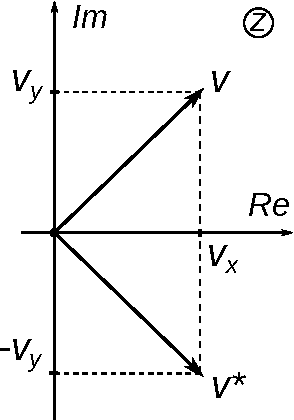
\includegraphics[width=0.3\linewidth]{../img/v_star.pdf}
	\caption{Определение комплексной скорости и её комплексно-сопряжённой величины}
	\label{fig:v_complex_dfn}
\end{figure}
					
Связь \textit{плоской потенциальной гидродинамической задачи} с теорией функций комплексного переменного (ТФКП) заключается в том, что соотношение
\[
w(z) = f(x+iy) = \varphi(x,y) + i  \psi(x,y)
\]
связывает аналитическую функцию $w(z)$ с определённой кинематической картиной течения и полем ($v_x$, $v_y$) с помощью аппарата ТФКП и наоборот.

\bigskip
Рассмотрим простейшие примеры.

\begin{problems}
\item 
\textbf{Однородное поступательное течение.}
Комплексный потенциал:
\[
	w(z) = a z,\quad
	a \in\mathbb{R}.
\]
		
Комплексная скорость:
\[
	\od{w}{z} = a = v_x - i v_y \Rightarrow
	v_x = a,\quad v_y = 0.
\]

Линии тока этого течения (при $a>0$) изображены на рис. \ref{fig:uniform_translation}.

\begin{figure}
	\centering
	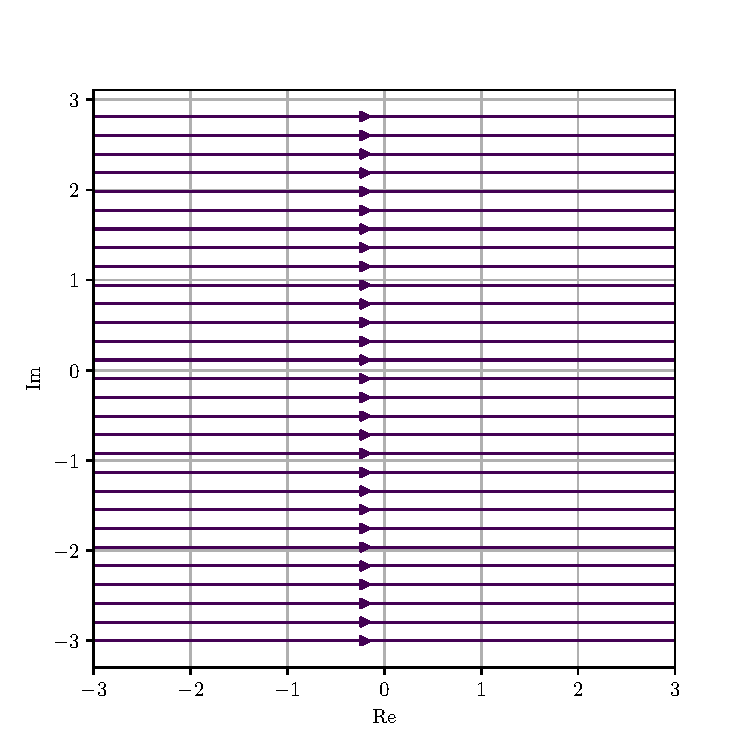
\includegraphics[width=0.45\textwidth]{../img/uniform_translation.pdf}
	\caption{Линии тока однородного поступательного движения при $a>0$}
	\label{fig:uniform_translation}
\end{figure}


\item 
\textbf{Источник и сток.} Комплексный потенциал:
\[
	w(z) = \frac{q}{2\pi}\ln(z-z_0),\quad
	q \in\mathbb{R}, z_0\in\mathbb{C}.
\]
			
Пусть $z=x+iy=re^{i\theta}$, тогда комплексная скорость (при $z_0 = 0$) имеет вид:
\[
\od{w}{z} = \frac{q}{2\pi}\frac{1}{z} \Rightarrow
\left\{
\begin{array}{l}
\displaystyle v_x = \frac{q}{2 \pi}\frac{x}{x^2+y^2} = \frac{q}{2\pi r}\cos\theta,\\
\displaystyle v_y = \frac{q}{2 \pi}\frac{y}{x^2+y^2} = \frac{q}{2\pi r}\sin\theta.
\end{array}
\right.
\]


Линии тока этого течения изображены на рис. \ref{fig:source_sink}.

\begin{figure}
	\centering
	\begin{tabular}{cc}
	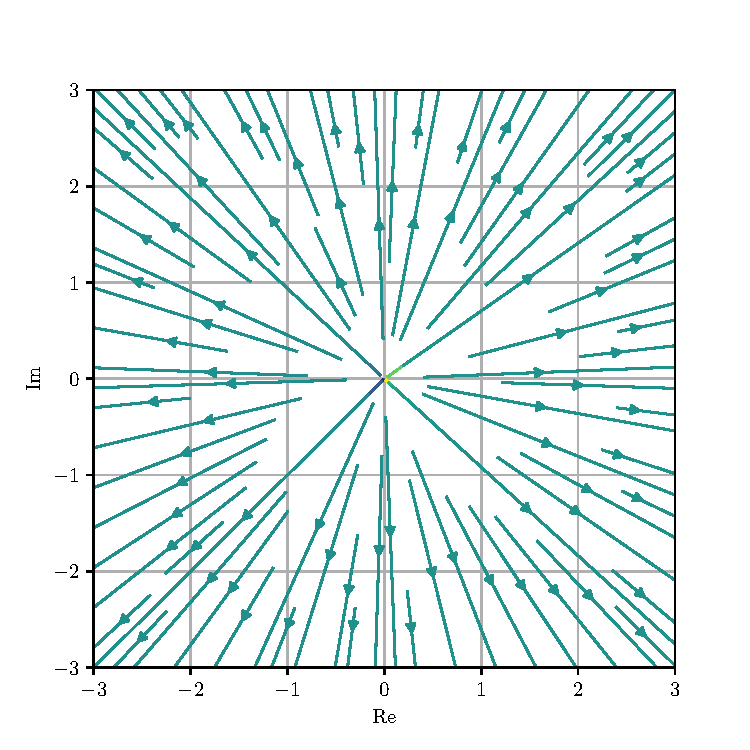
\includegraphics[width=0.45\textwidth]{../img/source.pdf} &
	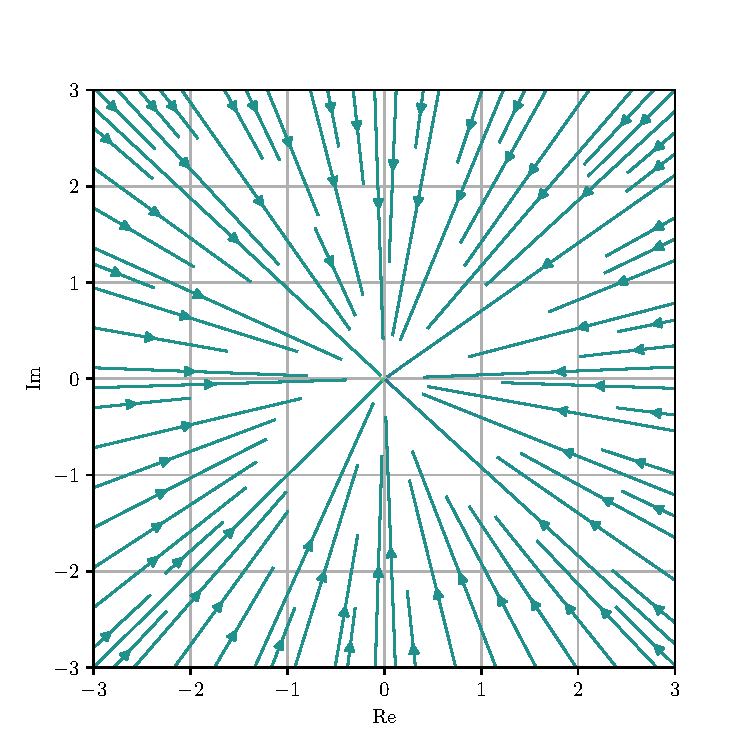
\includegraphics[width=0.45\textwidth]{../img/sink.pdf} \\
	а & б 
	\end{tabular}
	\caption{Линии тока источника ($q>0$) (a) и стока ($q<0$) (б)}
	\label{fig:source_sink}
\end{figure}

\item
\textbf{Вихрь.} Комплексный потенциал:
\[
	w(z) = \frac{\Gamma}{2\pi i}\ln(z-z_0),\quad
	\Gamma \in\mathbb{R}, z_0\in\mathbb{C}.
\]
			
Пусть $z=x+iy=re^{i\theta}$, тогда комплексная скорость (при $z_0=0$):
\[
	\od{w}{z} = \frac{\Gamma}{2\pi i}\frac{1}{z} \Rightarrow 
	\left\{
	\begin{array}{l}
		\displaystyle	v_x = -\frac{\Gamma}{2\pi}\frac{y}{x^2+y^2} = -\frac{\Gamma}{2\pi r}\sin\theta,\\
		\displaystyle	v_y = \frac{\Gamma}{2\pi}\frac{x}{x^2+y^2} = \frac{\Gamma}{2\pi r}\cos\theta.
	\end{array}
	\right.
\]

Линии тока этого течения изображены на рис. \ref{fig:rotor}.

\begin{figure}
	\centering
	\begin{tabular}{cc}
		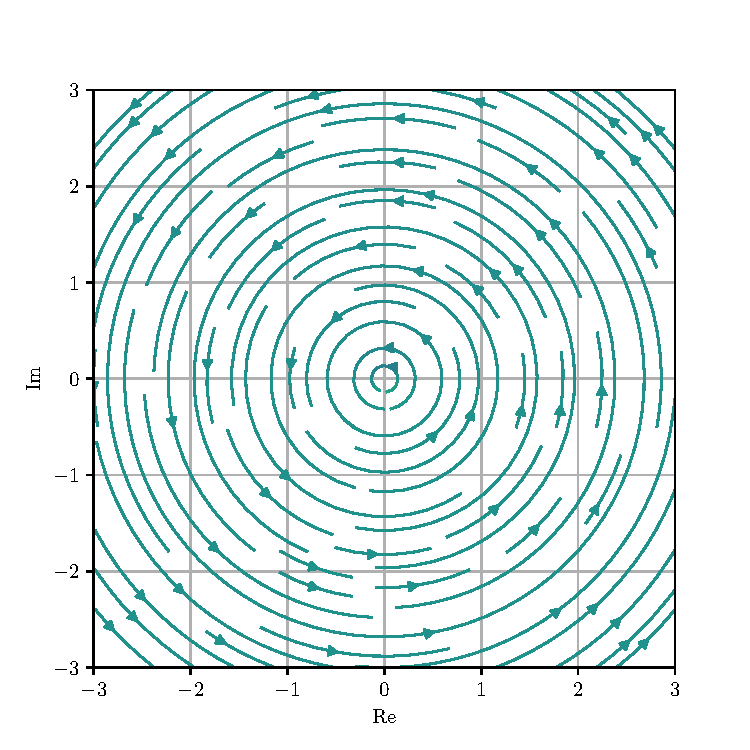
\includegraphics[width=0.45\linewidth]{../img/rot_Gamma_g_0.pdf} &
		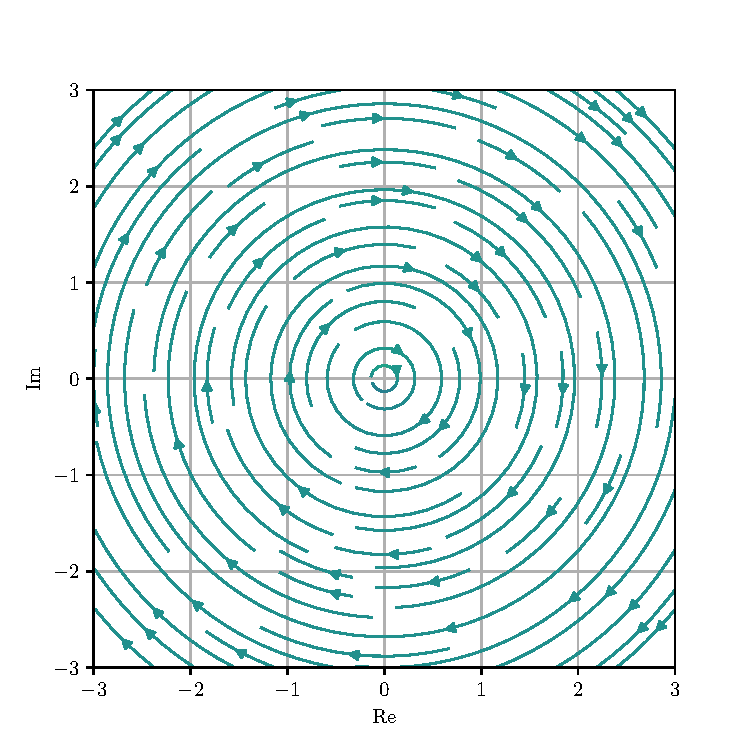
\includegraphics[width=0.45\linewidth]{../img/rot_Gamma_l_0.pdf} \\
		а & б 
	\end{tabular}
	\caption{Линии тока вихря, вращающегося в положительном ($\Gamma > 0$) (a) и отрицательном ($\Gamma < 0$) (б) направлениях}
	\label{fig:rotor}
\end{figure}

\item
\textbf{Диполь.}		
Комплексный потенциал:
\[
	w(z) = \frac{D e^{i\alpha}}{2\pi z},\quad
	D,\alpha \in\mathbb{R}.
\]
						
Пусть $z=x+iy=re^{i\theta}$, тогда комплексная скорость (при $\alpha=0$):
\[
	\od{w}{z} = -\frac{D}{2\pi}\frac{1}{z^2} \Rightarrow\displaystyle
	\left\{
	\begin{array}{l}
		v_x = -\displaystyle\frac{D}{2\pi r^2} \cos 2\theta,\\
		v_y = -\displaystyle\frac{D}{2\pi r^2} \sin 2\theta.
	\end{array}
	\right.
\]

Линии тока этого течения изображены на рис. \ref{fig:dipol}.

\begin{figure}
	\centering
	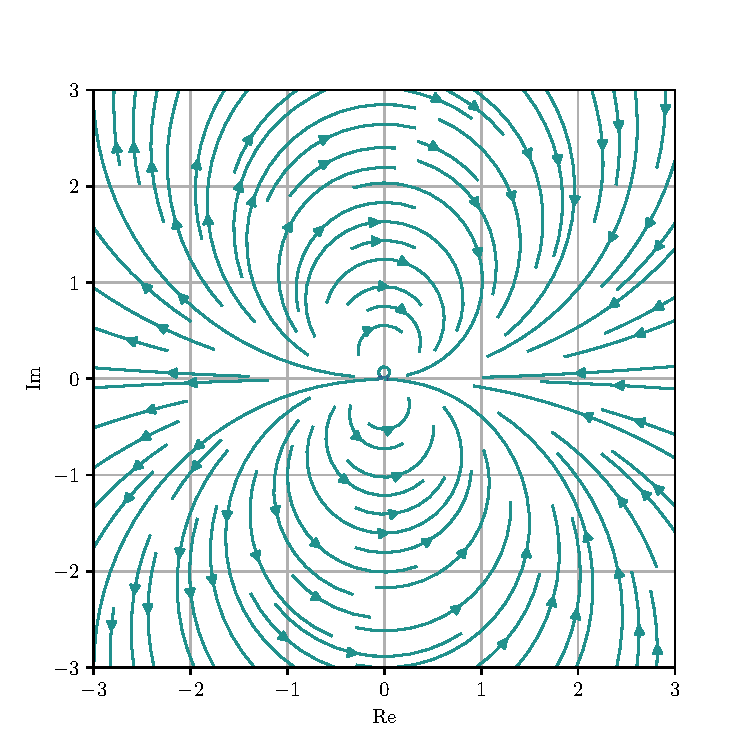
\includegraphics[width=0.45\linewidth]{../img/dipol.pdf}
	\caption{Линии тока диполя при $D>0$ и $\alpha = 0$}
	\label{fig:dipol}
\end{figure}
\end{problems}

\subsection{Построение потенциалов сложных течений}

Для моделирования течений, в которых присутствуют источники, стоки и другие элементарные течения применяется \textit{принцип суперпозиций}, заключающийся в следующем утверждении. Вследствие линейности уравнения неразрывности, если в области имеется несколько течений с потенциалами $w_1(z)$, $w_2(z)$, \ldots , $w_n(z)$, то общий потенциал всего течения в заданной точке равен сумме потенциалов всех течений, присутствующих в области:
\[
w(z) = w_1(z) + w_2(z) + \ldots + w_n(z).
\] 


Ещё один способ построения аналитических функций, описывающих плоские потенциальные течения ---  использовать \textit{метод конформных отображений} и \textit{теорему Римана о конформном отображение односвязных областей}. 

Основная идея заключается в построении конформного отображение физической плоскости $z$  на вспомогательную плоскость $\zeta$  с помощью аналитической функции $z=f(\zeta)$. Причём предполагается, что потенциал течения на вспомогательной плоскости известен $\psi(\zeta)$. Тогда искомый потенциал течения в физической плоскости  $\chi(z)$ будет выражаться из уравнений:
\[
\left\{
\begin{array}{l}
	\chi = \chi(f(\zeta)) = \psi(\zeta),\\
	z = f(\zeta).
\end{array}
\right.
\]
В этом случае комплексная скорость может быть найдена по формуле:
\[
v^* = \od{\chi}{z} = \od{\psi}{\zeta}  \od{\zeta}{z}.
\]


\subsection{Вычисление реакций и моментов сил, действующих на тело, при плоском потенциальном обтекании}
	

			
Для вычисления сил, моментов сил, действующих на выделенные контуры внутри области плоского потенциального течения, используют \textit{формулы Блазиуса -- Чаплыгина}:
\[
R^* = X - i Y = \frac{i\rho}{2} \oint\limits_C \left(\od{w}{z} \right)^2 dz,
\]	
\[
L = \Re \left[
-\frac{\rho}{2}\oint\limits_C \left(\od{w}{z} \right)^2 zdz
\right],
\]
где $R=X+i Y$ -- комплексная сила; $L$ -- величина главного момента; $\rho$ -- плотность жидкости; $C$ -- контур внутри или на границе области течения.

Также для вычисления реакций и момента главных сил можно использовать \textit{формулы Кутты -- Жуковского}. Если поток потенциален вне тела, которое можно заменить на конечное число источников, вихрей и диполей, лежащих внутри границы тела -- контура $C$, то
\[
R^* =  X - iY = i\rho\Gamma v_\infty^*,		
\]
\[
L = \Re \left[
-\rho v_\infty^*\sum\limits_{k=1}^m\Gamma_kb_k-i\rho M v_\infty^*
\right],
\]
где
$\Gamma_i$ -- циркуляции вихрей, находящихся в точках $b_i$ $(i=1,\ldots,m)$; $M$ -- суммарный момент источников и диполей; $\Gamma$ -- суммарная циркуляция вихрей, находящихся внутри тела.



\subsection{Задачи для самостоятельного решения}

\begin{problems}

	\item Установить связь функции тока с линиями тока.

	\item Рассмотреть плоское течение идеальной жидкости, задаваемое комплексным потенциалом $w(z) = Cz$, где $C = |C| e^{i \alpha}$.

	\item Для заданных комплексных потенциалов плоского течения идеальной жидкости:
		\begin{enumerate}
			\item 
			$
				w(z) = \ln \left( z^2 + \displaystyle\frac{1}{z^2} \right),
			$
			\item 
			$ 
			w(z) = \ln \left( 1 + \displaystyle\frac{1}{z^2} \right),
			$
		\end{enumerate}
	найти обильность $Q$ и построить качественную картину течения.
	
	\item 
	Границы какого геометрического объекта обтекаются идеальной несжимаемой жидкости с заданным комплексным потенциалом
	\[
		w(z)  = v_\infty z + v_\infty \frac{R^2}{z}?
	\]
	
	Влияет ли на граничные условия добавление потенциала циркуляции  $w(z) = \displaystyle\frac{\Gamma}{2 \pi i} \ln z$ при обтекании круга с центром в начале координат?
	
	
	\item В точках $z_1$ и $z_2$ заданы вихревые нити с циркуляциями $\Gamma_1$ и $\Gamma_2$. Требуется:
	\begin{enumerate}
		\item найти движение вихревых нитей в идеальной несжимаемой жидкости, 
		\item отдельно рассмотреть случай $\Gamma_1 = -\Gamma_2$.
	\end{enumerate}

	\item
	Какой контур обтекания соответствует комплексному потенциалу
	\[
	w(z) = z^2
	\]
	и каким будет итоговый комплексный потенциал, если в этот контур поместить источник?
	
	\item
	Идеальная несжимаемая жидкость занимает полупространство $y>0$. В точке  имеется нитевидный источник обильности $q$. Найти комплексный потенциал $w(z)$ и скорость $v$ стационарного плоского течения.
	
	\item
	Найти комплексный потенциал $w(z)$ и скорость $v$ стационарного плоского течения, создаваемого источником обильности $q$ при обтекании круга радиуса $R$, центр которого находится в начале координат. Источник расположен в точке $z_0$. 
	
	\item
	Пусть анализируемая 2D-система состоит из источника идеальной несжимаемой жидкости обильности $q$  и непроницаемой бесконечной линии раздела, находящейся на расстоянии $h$ от источника. Найти силу, действующую на источник.
	
	\item 
	Проанализировать циркуляцию при обтекании круга идеальной несжимаемой $2D$-жидкостью, включая описание критических точек как с графической, так и с позиции формул.
	
	\item 
	Построить потенциал обтекания эллипса на основе заданной функции отображения Жуковского $z = \zeta + c^2/\zeta$. Рассмотреть частный случай обтекания пластины.
	
	\item 
	Построить комплексный потенциал $w(z)$ обтекания непроницаемой параболы $y^2 = 2 p (x+p/2)$. Обтекание осуществляется по оси симметрии параболы $x$. Скорость на бесконечности $v_\infty$  задана.  Что за тип <<источника>> представляет член $\sqrt{pz}$? \textit{Указание: воспользоваться свойством функции тока $\psi$  на границе и формализмом распространения решения с границы на всю область.}
	
	\item
	Найти комплексный потенциал $w(z)$ и скорость $v$ при стационарном потенциальном обтекании идеальной несжимаемой жидкостью угла $\alpha$. Каким будет итоговый комплексный потенциал, если в этот контур поместить источник?
	
	\item
	Определить на основе постулата Жуковского-Чаплыгина циркуляцию, возникающую при обтекании идеальной несжимаемой жидкостью пластины длиной $2l$ под углом атаки $\alpha$.
	
\end{problems}

\section{Трёхмерные осесимметричные течения}


\subsection{Определения и постановка задачи для осесимметричных течений идеальной жидкости}



\begin{dfn}
Течение называется \alert{осесимметричным}, если существует такая прямая $l$, что во всех плоскостях, проходящих через $l$, картина течения одинакова и траектория жидкой частицы лежит в полуплоскостях, проходящих через $l$.
\end{dfn}

\begin{dfn}
Течение называется \alert{потенциальным}, если в некоторой области пространства можно определить потенциал $\varphi(t,x,y,z)$ такой, что
\[
	\vec{v} = \grad \varphi.
\]
\end{dfn}

Для трёхмерных потенциальных течений идеальной жидкости, определённых в некоторой области пространства, справедливо уравнение неразрывности:
\[
	\divo\vec{v}=\Delta\varphi = 0,\quad
	\vec{v}=\nabla \varphi
\]
и интеграл Коши
\[
	\pd{\varphi}{t} + \frac{\nabla\varphi^2}{2} + \frac{p}{\rho} = f(t)\footnote{Считаем, что поле внешних сил отстутствует.},
\]
где $p$ -- давление; $\rho$ -- плотность жидкости; $f(t)$ -- произвольная функция, определяемая из граничных и начальных условий. Интеграл Коши позволяет найти распределение давления по заданному потенциалу, известному из уравнения неразрывности ($\rho=const$).

Уравнение неразрывности в сферической системе координат ($r$,  $\lambda$, $\theta$) (рис.~\ref{fig:spherical_cylindrical_origin}а) в случае осесимметричного течения имеет вид\footnote{В следствие симметрии пренебрегли зависимостью $\varphi$ от $\lambda$.}:
\[
	\frac{1}{r^2 \sin\theta}
	\left\{
	\pd{}{r}\left( r^2 \sin\theta \pd{\varphi}{r} \right) + 
	\pd{}{\theta} \left( \sin\theta \pd{\varphi}{\theta} \right) 
%	+\pd{}{\lambda}\left( \frac{1}{\sin\theta} \pd{\varphi}{\lambda} \right)
	\right\}
	= 0,
\]
где
\[
	v_r = \pd{\varphi}{r},\quad
	v_\theta = \frac{1}{r}\pd{\varphi}{\theta}.
\]

\begin{figure}
	\centering
	\begin{tabular}{cc}
	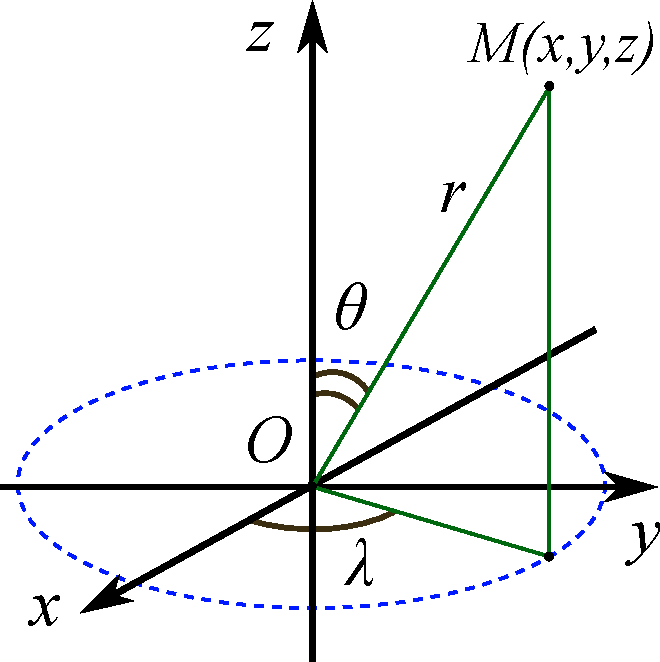
\includegraphics[width=0.45\linewidth]{../img/sphere_origin.pdf} & 
	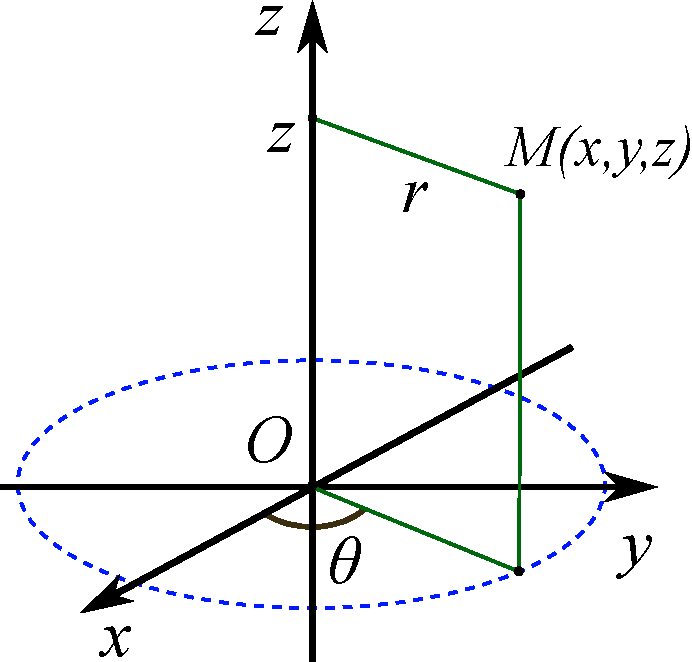
\includegraphics[width=0.45\linewidth]{../img/cylindrical_origin.pdf} \\
	а & б \\ 
	\end{tabular}
	\caption{Сферическая (а) и цилиндрическая (б) система координат}
	\label{fig:spherical_cylindrical_origin}
\end{figure}	


Уравнение неразрывности в цилиндрической системе координат ($r$, $\theta$, $z$)\footnote{В следствие симметрии пренебрегли зависимостью $\varphi$ от $\theta$.} (рис. \ref{fig:spherical_cylindrical_origin}б) в случае осесимметричного течения имеет вид:
\begin{equation}
\label{eq:mass_axis_symmetry_cylindrical}
\frac{1}{r}
\left\{
\pd{}{r}\left( r \pd{\varphi}{r} \right) + 
\pd{}{z}\left( r \pd{\varphi}{z} \right)
\right\}
= 0,
\end{equation}
где
\[
v_r = \pd{\varphi}{r},\quad
v_z =  \pd{\varphi}{z}.
\]

Из уравнение неразрывности в форме (\ref{eq:mass_axis_symmetry_cylindrical}) следует что
\[
	\pd{}{r}(r v_r)  = -\pd{}{z}(r v_z)
\]	
и существование полного дифференциала $\psi(r,z)$:
\[
	d\psi = r v_r dz - r v_z dr = \pd{\psi}{z} dz + \pd{\psi}{r} dr
\]


\begin{dfn}
Функцию $\psi(r,z)$  такую, что
\[
	v_r = \displaystyle\frac{1}{r}\pd{\psi}{z},\quad
	v_z = -\displaystyle\frac{1}{r}\pd{\psi}{r},
\]
называют \alert{функцией тока для осесимметричных течений}.	
\end{dfn}

Уравнения линий тока в случае осесимметричного течения в цилиндрической системе координат:
\[
\frac{dr}{v_r} = \frac{dz}{v_z},
\]
следовательно на линиях тока:
\[
d\psi = r (v_r dz - v_z dr) = 0
\]
и $\psi = const$.

Соотношения
\[
	\pd{\varphi}{r} = \frac{1}{r}\pd{\psi}{z},\quad
	\pd{\varphi}{z} = -\frac{1}{r}\pd{\psi}{r}
\]
связывают функцию тока и потенциал для осесимметричных течений. Полученные соотношения \alert{отличаются} от условий Коши -- Римана (\ref{eq:Cauchi_Riman}), а уравнение для функции тока:
\[
	\pdk{\psi}{r}+\pdk{\psi}{z} - \frac{1}{r}\pd{\psi}{r} = 0
\]
не является уравнением Лапласа, записанным в цилиндрической системе координат. 
В случае осесимметричных течений не работают методы ТФКП. В этом случае может быть применен \alert{метод источников и стоков} и \alert{принцип суперпозиций}. 
		
Для моделирования течений, потенциалы которых известны применяется \textit{принцип суперпозиций}, заключающийся в следующем утверждении. Вследствие линейности уравнения неразрывности, если в области имеется несколько течений с потенциалами $\varphi_1(x,y)$, $\varphi_2(x,y)$, \ldots, $\varphi_n(x,y)$, то общий потенциал всего течения в заданной точке равен сумме потенциалов всех течений, присутствующих в области:
\[
\varphi(x,y) = \varphi_1(x,y) + \varphi_2(x,y) + \ldots + \varphi_n(x,y)
\] 		
или интегралу от непрерывно распределенных потенциалов в некоторой области пространства.

		
	%\end{exampleblock}
	%
	%
	%}
%
%\frame{
	%\frametitle{Связь между функций тока и потенциалом}
	%
	%\begin{exampleblock}{Предпосылки}
	%	\parbox{\textwidth}{
		%		\[
		%		d\psi = 
		%		\pd{\psi}{r}dr+\pd{\psi}{z}dz = 
		%		-r\left( \pd{\varphi}{z}dr - \pd{\varphi}{r} dz \right),
		%		\]
		%		\[
		%		d\varphi = 
		%		\pd{\varphi}{r}dr+\pd{\varphi}{z}dz = 
		%		\frac{1}{r}\left( \pd{\psi}{z}dr - \pd{\psi}{r} dz \right).
		%		\]
		%		
		%	}
	%\end{exampleblock}
	%
	%\begin{exampleblock}{Искомые соотношения}
	%	\parbox{\textwidth}{
		%		
		%		\[
		%		\psi(r,z) = \psi(r_0,z_0) + \int\limits_{r_0,z_0}^{r,z} r \left(
		%		\pd{\varphi}{r} dz - \pd{\varphi}{z} dr		
		%		\right),
		%		\]
		%		\[
		%		\varphi(r,z) = \varphi(r_0,z_0) + \int\limits_{r_0,z_0}^{r,z} \frac{1}{r} \left(
		%		\pd{\psi}{z} dr - \pd{\psi}{r} dz		
		%		\right).
		%		\]
		%	}
	%\end{exampleblock}
	%
	%
	%}
%


%\frame{
%\frametitle{ Источник в пространстве}
%
%\begin{exampleblock}{Сферически симметричное течение}
%	\parbox{\textwidth}{
%		\[
%		\varphi = \varphi(r) \quad \Rightarrow \quad
%		\pd{}{r}\left( r^2 \od{\varphi}{r} \right) = 0
%		\]
%		
%	}
%\end{exampleblock}\pause
%
%\begin{exampleblock}{Потенциал источника, расположенного в точке с координатами $(a,b,c)$}
%	\parbox{\textwidth}{
%		\[
%		\varphi(x,y,z) = -\frac{q}{4\pi \sqrt{(x-a)^2+(y-b)^2+(z-c)^2}}
%		\]
%		
%	}
%\end{exampleblock}\pause
%
%\begin{exampleblock}{Расход жидкости через любую поверхность, охватывающую центр источника S}
%	\parbox{\textwidth}{
%		\[
%		q = \int\limits_S v_n dS = \int\limits_S \pd{\varphi}{n} dS
%		\]
%		
%	}
%\end{exampleblock}
%}
%
%\frame{
%\frametitle{Диполь в пространстве}
%
%\begin{exampleblock}{Потенциал}
%	\parbox{\textwidth}{
%		Рассмотрим источник и сток одной и той же обильности $q$, которые находятся на оси $Oz$ на расстоянии $l$ друг от друга. Тогда их суммарный потенциал будет иметь вид
%		\[
%		\varphi =  -\frac{q}{4\pi \sqrt{x^2+y^2+(z-l/2)^2}} +
%		\frac{q}{4\pi \sqrt{x^2+y^2+(z+l/2)^2}}.
%		\]\pause
%		
%		При переходе к пределу при $l \to 0 $, а $q \to \infty$, причем $ql = M$, получится предельный потенциал
%		\[
%		\varphi = -\frac{Mz}{4\pi r^3}, \quad \text{или} \quad
%		\varphi = -\frac{M}{4\pi} \pd{}{l}\left(\frac{1}{r}\right),
%		\]
%		где $M$ -- момент диполя; $l$ -- направление оси диполя.
%	}
%\end{exampleblock}
%
%}
%
%\frame{
%\frametitle{ Обтекание сферы }
%
%\begin{exampleblock}{Постановка}
%	\smallskip
%	\parbox{\textwidth}{
%		Требуется найти распределение скорости и давления при потенциальном обтекании сферы радиуса $R$, движущейся поступательно вдоль оси $Oz$ со скоростью $u$ в потоке идеальной жидкости, имеющей на бесконечности скорость $V$, направленную вдоль оси $Oz$, и давление $p_\infty$.
%	}
%\end{exampleblock}
%
%\centering
%\includegraphics[width=0.7\textwidth]{../img/sphere.pdf}
%
%
%
%
%}
%
%\frame{
%\frametitle{ Математическая постановка }
%\begin{exampleblock}{Основные уравнения}
%	\parbox{\textwidth}{
%		В сферической системе координат пренебрегаем зависимостью от $\lambda$. Тогда для функции $\varphi = \varphi(r,\theta)$ запишем уравнение неразрывности:
%		\[
%		\pd{}{r}\left( r^2 \sin\theta \pd{\varphi}{r} \right) +
%		\pd{}{\theta} \left( \sin\theta\pd{\varphi}{\theta} \right) = 0.
%		\]
%	}
%\end{exampleblock}
%
%\begin{exampleblock}{Граничные условия на сфере}
%	\parbox{\textwidth}{
%		\[
%		v_n = \left. \pd{\varphi}{n} \right|_{r=R} = u \cos\theta
%		\]
%	}
%\end{exampleblock}
%
%\begin{exampleblock}{Граничные условия на бесконечности}
%	\parbox{\textwidth}{
%		\[
%		v_r = \left. \pd{\varphi}{r} \right|_{r\to\infty} = V \cos\theta,\quad
%		v_\theta = \frac{1}{r} \left. \pd{\varphi}{\theta} \right|_{r\to\infty} = -V \sin\theta.
%		\]
%	}
%\end{exampleblock}
%}
%
%\frame{
%\frametitle{ Решение задачи обтекания сферы }
%
%\begin{exampleblock}{Упрощение}
%	\parbox{\textwidth}{
%		Пусть $\varphi(r,\theta) = Q(r) \cos\theta$, тогда уравнение неразрывности будет иметь вид:
%		\[
%		r^2 \odk{Q}{r}{2} + 2r\od{Q}{r} - 2Q = 0.
%		\]
%	}
%\end{exampleblock}
%
%\begin{exampleblock}{Аналитическое решение}
%	\parbox{\textwidth}{
%		\[
%		\varphi(r,\theta) = \left(Vr + \frac{V-u}{2} \frac{R^3}{r^2}\right) \cos\theta
%		\]
%		можно переписать в виде:
%		\[
%		\varphi = Vz- \frac{R^3}{2}(V-u) \pd{}{z}\left( \frac{1}{r} \right).
%		\]
%		
%		Это сумма потенциала поступательного движения потока со скоростью $V$ и потенциала диполя с моментом  $M = 2\pi R^3 (u-V)$.
%	}
%\end{exampleblock}
%
%
%}
%
%\frame{
%\frametitle{ Обтекание покоящейся сферы }
%
%\parbox{\textwidth}{
%	Если $u=0$, тогда
%	\[
%	\varphi = V \left(r+\frac{1}{2}\frac{R^3}{r^2}\right) \cos\theta
%	\]
%	и
%	\[
%	v_r = V \left(1 - \frac{R^3}{r^3}\right) \cos\theta,\quad
%	v_\theta = -V \left(1 + \frac{R^3}{2r^3}\right) \sin\theta.
%	\]
%	
%	Максимальное значение скорости на поверхности сферы достигается в точках $\theta=\pm\pi/2$ и равно $3/2V$.
%	
%}
%
%
%
%}
%
%\frame{
%\frametitle{ Парадокс Даламбера для покоящейся сферы}
%
%\begin{exampleblock}{Интеграл Бернулли}
%	\parbox{\textwidth}{
%		Так как течение потенциально и стационарно, то 
%		\[
%		\frac{v^2}{2} + \frac{p}{\rho} = \frac{V^2}{2} + \frac{p_\infty}{\rho}.
%		\]
%		
%	}
%\end{exampleblock}
%
%\begin{exampleblock}{Выражение для давления}
%	\parbox{\textwidth}{
%		\[
%		\frac{p-p_\infty}{\rho} = \frac{V^2}{2}\left( 1- \frac{9}{4} \sin^2 \theta \right)
%		\]
%		
%	}
%\end{exampleblock}
%
%\parbox{\textwidth}{
%	Суммарная сила, вызванная давлением потенциального течения жидкости на покоящуюся сферу, равна 0 вследствие симметрии распределения сил давления. Это называется \alert{парадоксом Даламбера}.
%}
%
%
%}
%
%\frame{
%\frametitle{ Функция тока для осесимметричных течений }
%
%\begin{exampleblock}{Уравнение неразрывности в цилиндрической системе координат с осевой симметрией в переменных $(r,z)$}
%	\parbox{\textwidth}{
%		\[
%		\divo \vec{v} =\frac{1}{r} \left( \pd{}{r}(r v_r) + \pd{}{z}(r v_z)\right) = 0\quad \Rightarrow \quad
%		\pd{}{r}(r v_r)  = -\pd{}{z}(r v_z)
%		\]	
%	}
%\end{exampleblock}
%\begin{exampleblock}{Существование полного дифференциала}
%	\parbox{\textwidth}{
%		\[
%		d\psi = r v_r dz - r v_z dr = \pd{\psi}{z} dz + \pd{\psi}{r} dr
%		\]
%		является полным дифференциалом (см. теорию про интегрирующий множитель).
%	}
%\end{exampleblock}
%\begin{exampleblock}{Определение}
%	\parbox{\textwidth}{
%		Функцию $\psi(r,z)$  такую, что
%		$
%		v_r = \displaystyle\frac{1}{r}\pd{\psi}{z}$,
%		$v_z = -\displaystyle\frac{1}{r}\pd{\psi}{r}
%		$,
%		называют \alert{функцией тока для осесимметричных течений}.	
%	}
%\end{exampleblock}
%}
%
%\frame{
%\frametitle{Свойства функции тока }
%
%\begin{exampleblock}{Постоянство на линиях тока}
%	\smallskip
%	\parbox{\textwidth}{
%		Уравнение линий тока в случае осесимметричного течения:
%		\[
%		\frac{dr}{v_r} = \frac{dz}{v_z},
%		\]
%		поэтому на линиях тока: 
%		\[
%		v_r dz - v_z dr = 0,
%		\]
%		следовательно
%		\[
%		d\psi = r (v_r dz - v_z dr) = 0
%		\]
%		и $\psi = const$.
%		
%		
%	}
%\end{exampleblock}
%
%}
%
%\frame{
%\frametitle{ Свойства функции тока }
%
%\begin{columns}
%	\begin{column}{0.35\textwidth}
%		\includegraphics[width=\textwidth]{../img/streamfunction_flow.pdf}
%	\end{column}
%	\begin{column}{0.65\textwidth}
%		
%		\begin{exampleblock}{Поток жидкости через поверхность $S$}
%			\parbox{\textwidth}{
%				
%				\[
%				\int\limits_S \vec{v}\cdot\vec{n} ds = 
%				\int\limits_{0}^{2\pi}  \int\limits_B^A \left( v_z n_z + v_r n_r \right) r d\theta dl = 
%				\]
%				\[
%				=
%				2 \pi \int\limits_0^{l_0} \left( \left(-\frac{1}{r}\pd{\psi}{r} \right) \left(-\pd{r}{l}\right) + \frac{1}{r}\pd{\psi}{z} \pd{z}{l} \right) r dl=
%				\]
%				\[
%				=
%				2\pi\int\limits_0^{s_0} \od{}{l} \psi(r(l),z(l)) dl = 2\pi(\psi(A) - \psi(B)),
%				\]
%				\[
%				r=r(l),\quad z=z(l),
%				\]
%				\[
%				(r,z)|_{l=0} = B,\quad
%				(r,z)|_{l=l_0} = A.
%				\]
%				
%			}
%		\end{exampleblock}			
%	\end{column}
%\end{columns}
%}
%\frame{
%\frametitle{ Связь функции тока и потенциала для осесимметричных течений}
%
%\begin{exampleblock}{Соотношения}
%	\parbox{\textwidth}{
%		\[
%		\pd{\varphi}{r} = \frac{1}{r}\pd{\psi}{z},\quad
%		\pd{\varphi}{z} = -\frac{1}{r}\pd{\psi}{r}
%		\]
%		Полученные соотношения \alert{отличаются} от условий Коши -- Римана.
%	}
%\end{exampleblock}\pause
%
%\begin{exampleblock}{Уравнение для функции тока}
%	\parbox{\textwidth}{
%		\[
%		\pdk{\psi}{r}+\pdk{\psi}{z} \alert{-} \frac{1}{r}\pd{\psi}{r} = 0
%		\]
%		
%		Полученное соотношение не является уравнением Лапласа, записанным в цилиндрической системе координат. В случае осесимметричных течений не работают методы ТФКП. В этом случае может быть применен \alert{метод источников и стоков}. 
%	}
%\end{exampleblock}
%
%
%}
%
%\frame{
%\frametitle{Связь между функций тока и потенциалом}
%
%\begin{exampleblock}{Предпосылки}
%	\parbox{\textwidth}{
%		\[
%		d\psi = 
%		\pd{\psi}{r}dr+\pd{\psi}{z}dz = 
%		-r\left( \pd{\varphi}{z}dr - \pd{\varphi}{r} dz \right),
%		\]
%		\[
%		d\varphi = 
%		\pd{\varphi}{r}dr+\pd{\varphi}{z}dz = 
%		\frac{1}{r}\left( \pd{\psi}{z}dr - \pd{\psi}{r} dz \right).
%		\]
%		
%	}
%\end{exampleblock}
%
%\begin{exampleblock}{Искомые соотношения}
%	\parbox{\textwidth}{
%		
%		\[
%		\psi(r,z) = \psi(r_0,z_0) + \int\limits_{r_0,z_0}^{r,z} r \left(
%		\pd{\varphi}{r} dz - \pd{\varphi}{z} dr		
%		\right),
%		\]
%		\[
%		\varphi(r,z) = \varphi(r_0,z_0) + \int\limits_{r_0,z_0}^{r,z} \frac{1}{r} \left(
%		\pd{\psi}{z} dr - \pd{\psi}{r} dz		
%		\right).
%		\]
%	}
%\end{exampleblock}
%
%
%}
%
%
%\frame{
%\frametitle{ Функция тока  для простейших осесимметричных течений}
%
%\begin{exampleblock}{Поступательное движение}
%	\parbox{\textwidth}{
%		
%		\[
%		\varphi = V z \quad\Rightarrow\quad
%		\psi = -\frac{V}{2}r^2
%		\]
%	}
%\end{exampleblock}
%
%\begin{exampleblock}{Источник}
%	\parbox{\textwidth}{
%		\[
%		\varphi = -\frac{q}{4\pi} \frac{1}{r^2+z^2}\quad\Rightarrow\quad
%		\psi = \frac{q}{4\pi}\frac{z}{\sqrt{r^2+z^2}} + C
%		\]	
%	}
%\end{exampleblock}
%\begin{exampleblock}{Диполь}
%	\parbox{\textwidth}{
%		\[
%		\varphi =  -\frac{M}{4\pi} \frac{z}{r^3}\quad\Rightarrow\quad
%		\psi =  -\frac{M}{4\pi} \frac{r^2}{(\sqrt{r^2+z^2})^3}+C
%		\]
%	}
%\end{exampleblock}
%
%
%}


\subsection{Задачи для самостоятельного решения}

\begin{problems}
	
	\item 
	Как преобразуются условия Коши-Римана в случае цилиндрических и сферических координат? Как выглядят операторы дифференциальных уравнений в постановке задач на потенциал и функцию тока (задачи Дирихле, Неймана)?
	
	\item Показать, что поток жидкости через поверхность, образованную вращением дуги, равен разности значений функции тока на концах этой дуги.
	
	\item 
	Для шара, двигающегося с ускорением в идеальной несжимаемой жидкости, определить силу, действующую на жидкость. \textit{Указание: воспользоваться уравнением Коши-Лагранжа после определения потенциала жидкости.}
	
	\item 
	Найти частоту колебаний шарика, находящегося в идеальной несжимаемой жидкости в случаях: 
	\begin{enumerate}
		\item шарик колеблется в плоскости, перпендикулярной вектору силы тяжести,
		\item шарик колеблется в поле силы тяжести.
	\end{enumerate}
	
	\item 
	Сферический пузырек всплывает в идеальной несжимаемой жидкости с плотностью $\rho$. Ускорение свободного падения $g$. Определить ускорение пузырька. Массой пузырька можно пренебречь.
	
	\item
	Сферический пузырек приводится в движение жидкостью. Ускорение жидкости вдали от пузырька равно $w$. Определить ускорение пузырька. Масса пузырька пренебрежимо мала, размер постоянен.
	
\end{problems}	

\section{Динамика вязкой жидкости}

\subsection{Задачи для самостоятельного решения}

\begin{enumerate}
	
	\item Найдите вектор скорости, давление, вектор вихря и силу Стокса при обтекании шара вязкой жидкостью в приближении Стокса.
	
	{\small
	\textit{Указание.}	
	
	Решение (поиск констант) предлагается искать следующим образом: подействуйте ротором на уравнение количества движения в приближении Стокса, что приведет к уравнению на вектор вихря, затем воспользуйтесь соображением симметрии для вектора вихря, далее, найдите вектор вихря с точностью до константы, решая дифференциальное уравнение, затем, пользуясь уравнением неразрывности и разложением в ряд для скоростей в сферических координатах (по расстоянию от центра шара), найдите компоненты скоростей с учетом граничного условия. Определив давление, найдите силу Стокса.  \newline		
	Решение  также можно искать следующим образом: подействуйте оператором дивергенции на уравнение количества движения с целью выделения уравнения на давление. Это даст множество решений, но из лекции мы знаем какое взять. Почему член  не входит в выражение для давления? Помимо условий на границе шара, используйте уравнение неразрывности для получения условий на неизвестные константы. При нахождении констант не забудьте также про константу при давлении. Почему член  не входит в выражение для скорости? Почему член  входит в выражение для скорости и к чему это приводит (относительно обтекания сферы идеальной жидкостью посмотреть)? Как симметрия задачи оказывает влияние на составление членов, потенциально подходящих под решение?
	}

	\item 
	Проанализировать поведение найденного поля скоростей при отдалении от шара. Почему наблюдается такое поведение скоростей? Что следует сделать, чтобы уточнить полученное решение? 
	
	\item
	Показать, что в вязкой жидкости происходит диссипация энергии.
	 
	{\small \textit{Указание:} показать, что работа, совершаемая над жидкостью, не целиком идёт на изменение кинетической энергии.}

\end{enumerate}

\section{$\Pi$-теорема}

\subsection{Задачи для самостоятельного решения}

\begin{enumerate}
	
	\item Используя $\Pi$-теорему, определить силу сопротивления шара при его внедрении с постоянной скоростью $v$ в полупространство, заполненное вязкой несжимаемой жидкостью. Рассмотреть предельные случаи $v \to 0$, $v \to \infty$. Радиус шара известен.
	
	\item
	Используя  $\Pi$-теорему, определить силу сопротивления, действующую на шар, движущийся в вязкой, несжимаемой бесконечной жидкости. Рассмотреть предельные случаи $v \to 0$, $v \to \infty$. Основные параметры системы считать заданными.
	
	\item
	Задача о точечном взрыве. В некоторой точке выделилось количество энергии $E$ . Определить зависимости скорости $D$ и координаты $R$ ударной волны от времени $t$, а также скорость $v_2$, плотность $\rho_2$ и давление $p_2$ за ударной волной. 

\end{enumerate}

\section{Одномерные изоэнтропические течения идеального газа }

\subsection{Задачи для самостоятельного решения}

\begin{enumerate}
	
	\item Пользуясь методом характеристик, повторить вывод инвариантов Римана и характеристических направлений на основе изоэнтропического приближения одномерной газовой динамики.
	
	\item
	В момент $t=0$  покоящийся газ с параметрами $v_0 = 0$, $p_0$, $\rho_0$ находится в трубе при $x<0$. Справа в трубе вакуум. Найти $v(x,t)$, $\rho(x,t)$, $p(x,t)$, $T(x,t)$, $c(x,t)$ при истечении газа в вакуум. Сравнить полученную максимальную скорость истечения газа c максимальной скоростью истечения газа в вакуум в стационарном случае.
	
	\item 
	В цилиндр, заполненный покоящимся воздухом с параметрами $v_0 = 0$, $\rho=\rho_0$, $p=p_0$, вдвигается поршень с постоянным ускорением $a$. Найти момент возникновения ударной волны $t^*$.
	
	\item
	Определить закон движения поршня площадью $S$ и массой $m$, выталкиваемого газом с начальными параметрами $v_0=0$, $p_0$, $\rho_0$ в вакуум (см. иллюстрацию).

	\begin{figure}[h!]
		\centering
		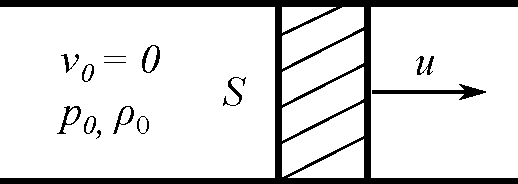
\includegraphics[width=0.5\textwidth]{../img/piston_u.pdf}
	\end{figure}
	
	\item 
	Из трубы, заполненной при $x>0$ газом с параметрами  $v_0=0$, $p_0$, $\rho_0$, начинает выдвигаться поршень с постоянной скоростью $u$. Определить движение газа.

\end{enumerate}

\end{document}